\section{Theorie}
\label{sec:Theorie}

\subsection{sec:Austrittsarbeit und Energie}
\label{sec:Austrittsarbeit und Energie}
Werden Metalle erhitzt, treten aus der Oberfläche Elektronen aus.
Diese Elektronenemission wird als \textit{glühelektrischer Effekt} bezeichnet.
Werden Metalle erhitzt, treten aus der
\begin{wrapfigure}{r}{0.4\linewidth}
    \caption{Darstellung eines sogenannten Potentialtopfes}\label{fig:Potentialtopf}
    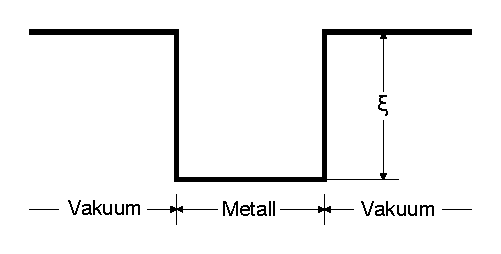
\includegraphics[width=\linewidth]{pictures/Potentialtopf.pdf}
\end{wrapfigure} 
Oberfläche Elektronen aus.
Werden Metalle erhitzt, treten aus der Oberfläche Elektronen aus.
Dafür müssen diese aber zunächst die \textit{Austrittsarbeit} $e_0 \xi$ leisten.
Dabei sit $\xi$ das Potential, welches in \hyperref[fig:Potentialtopf]{Abbildung \ref{fig:Potentialtopf}} anschaulich dargestellt wurde, und
$e_0$ ist die Elementarladung.
Elektronen haben immer eine Energie die von null verschieden ist.
Das wird durch das Pauliprinzip auch am absoluten Temperaturnullpunkt garantiert.
Die Wahrscheinlichkeit , dass im thermischen Gleichgewicht ein Zustand mit einer Energie $E$ besetzt ist, wird durch die
\textit{Fermi-Dirac'sche Verteilungsfunktion}
\begin{equation}
    f(E)=\frac{1}{\exp \left(\frac{E-\zeta}{k T}\right)+1}
\end{equation}
beschrieben. Dabei beschreibt $\zeta$ die \textit{Fermische Grenzenergie}, $k$ die Boltzmann-Konstante und $T$ die Temperatur.

\subsection{Richardson-Gleichung}
\label{eq:Richardson}
Die Sättigungsstromdichte wird durch die sogenannte \textit{Richardson-Gleichung} \cite{v504} beschrieben. Sie lautet
\begin{equation}
    j_{S}(T)=4 \pi \frac{e_{0} m_{0} k^{2}}{h^{3}} T^{2} \exp \left(\frac{-e_{0} \Phi}{k T}\right) .
\end{equation}
\subsection{Hochvakuum-Diode}
Für die Messung des Sättigungsstromes ist eine Hochvakuum-Diode nötig, da sonst die freien Elektronen mit den Gasmolekülen wechselwirken würden.
\begin{figure} [H]
    \center
    \caption{Schematische Darstellung einer Hochvakuum-Diode}\label{fig:Diode}
    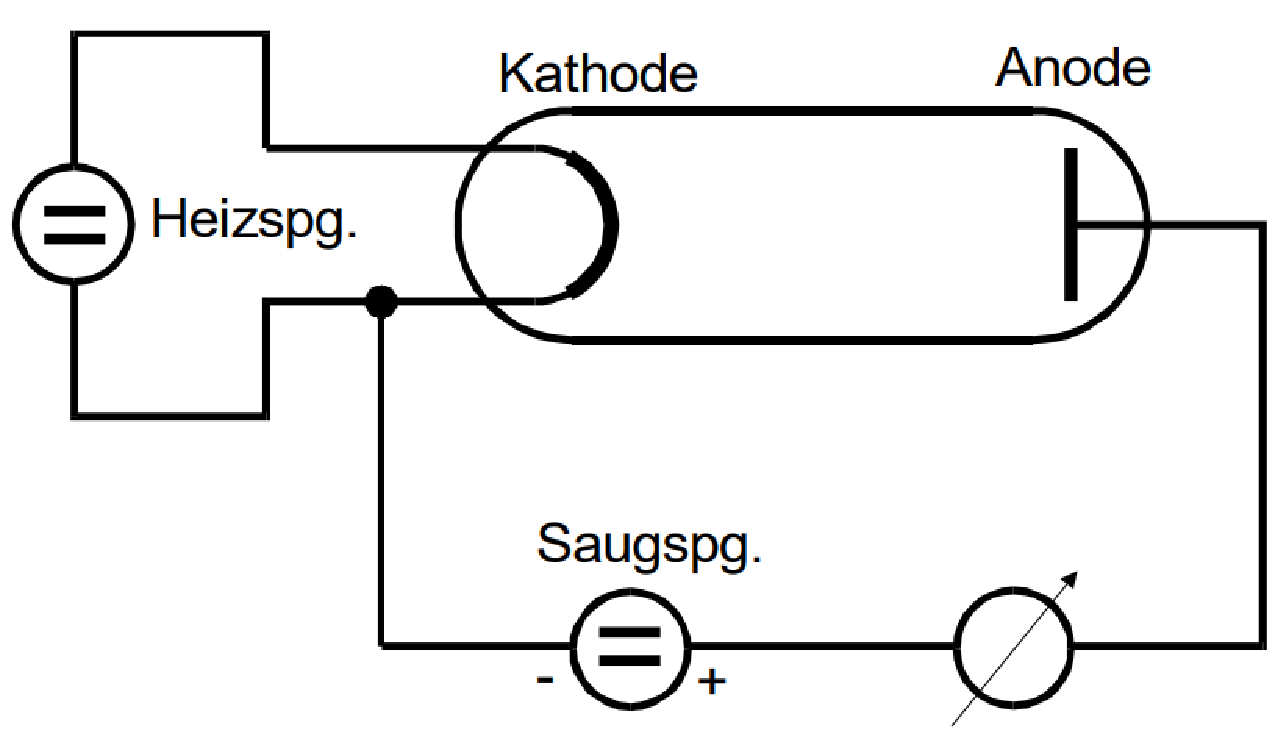
\includegraphics[width=0.5\linewidth]{pictures/Diode.pdf}
\end{figure}
Innerhalb der Diode, dargestellt in \hyperref[fig:Diode]{Abbildung \ref{fig:Diode}} wird durch die Anode ein elektrisches Feld angelegt, durch welches die Elektronen \enquote{abgesaugt} werden.
Die Elektronen werden durch die Heizspannung an der Kathode abgegeben.

\subsection{Die Langmuir-Schottkysche Raumladungsgleichung}
Wird der Anodenstrom bei einem Aufbau wie in \hyperref[fig:Diode]{Abbildung \ref{fig:Diode}} gemessen, lässt sich feststellen,
dass dieser abhängig von der Anodenspannung ist.
Erst mit höherer Spannung erreichen annähernd alle ELektionen die Anode.
Da es sich bei der Elektronenbewegung um eine beschleunigte Bewegung handelt, ist das Ohmsche Gesetz hier nicht gültig.
Durch die beschleunigte Bewegung wird die Raumladungsdichte zur Anode hin geringer.
Dadurch wird der Verlauf der Feldlinien, also der Feldstärke, beeinflusst.
Hinzu kommt, dass durch diesen Effekt die Abschirmung des Feldes der Kathode, wodurch die emittierten
Elektronen nicht mehr vom Anodenfeld erfasst werden.
Deshalb ist der gemessene Diodenstrom geringer als der erwartete Sättigungsstrom.
Die Stromdichte lässt sich durch die sogenannte \textit{Langmuir-Schottkysche Raumladungsgleichung} 
\begin{equation}
    j=\frac{4}{9} \varepsilon_{0} \sqrt{\frac{2 e_{0} }{ m_{0}}} \frac{V^{\frac{3}{2}}}{a^{2}}
\end{equation}
beschreiben. Der Gültigkeitsbereich wird \textit{Raumladungsgebiet} genannt.

\subsection{Das Anlaufstromgebiet einer Hochvakuum-Diode}
Selbst bei einer Anodenspannung von $U_A = 0$ lässt sich ein Anodenstrom messen.
Dies wird durch die Eigengeschwindigkeit der Elektronen bei verlassen der Kathode erklärt.
Selbst bei einem geringem Gegenfeld kommen einige Elektronen an der Anode an, weshalb sie die Energie $E \geq e_0 (\phi_A + U_A)$ haben müssen.
Dieses Gegenfeld wird als Anlaufstrom bezeichnet.
Der Verlauf des Anodenstromgebietes lässt sich durch
\begin{equation}
    \mathrm{j}(\mathrm{V})=\mathrm{j}_{0} \exp \left(-\frac{\mathrm{e}_{0} \phi_{\mathrm{A}}+\mathrm{e}_{0} \mathrm{~V}}{\mathrm{kT}}\right)=\text { const } \exp \left(-\frac{\mathrm{e}_{0} \mathrm{~V}}{\mathrm{kT}}\right)
\end{equation}
beschreiben.

\subsection{Die Kennlinie der Hochvakuum-Diode}
\begin{figure}
    \center
    \caption{Kennlinie einer Hochvakuum-Diode}\label{fig:KennlinieTheorie}
    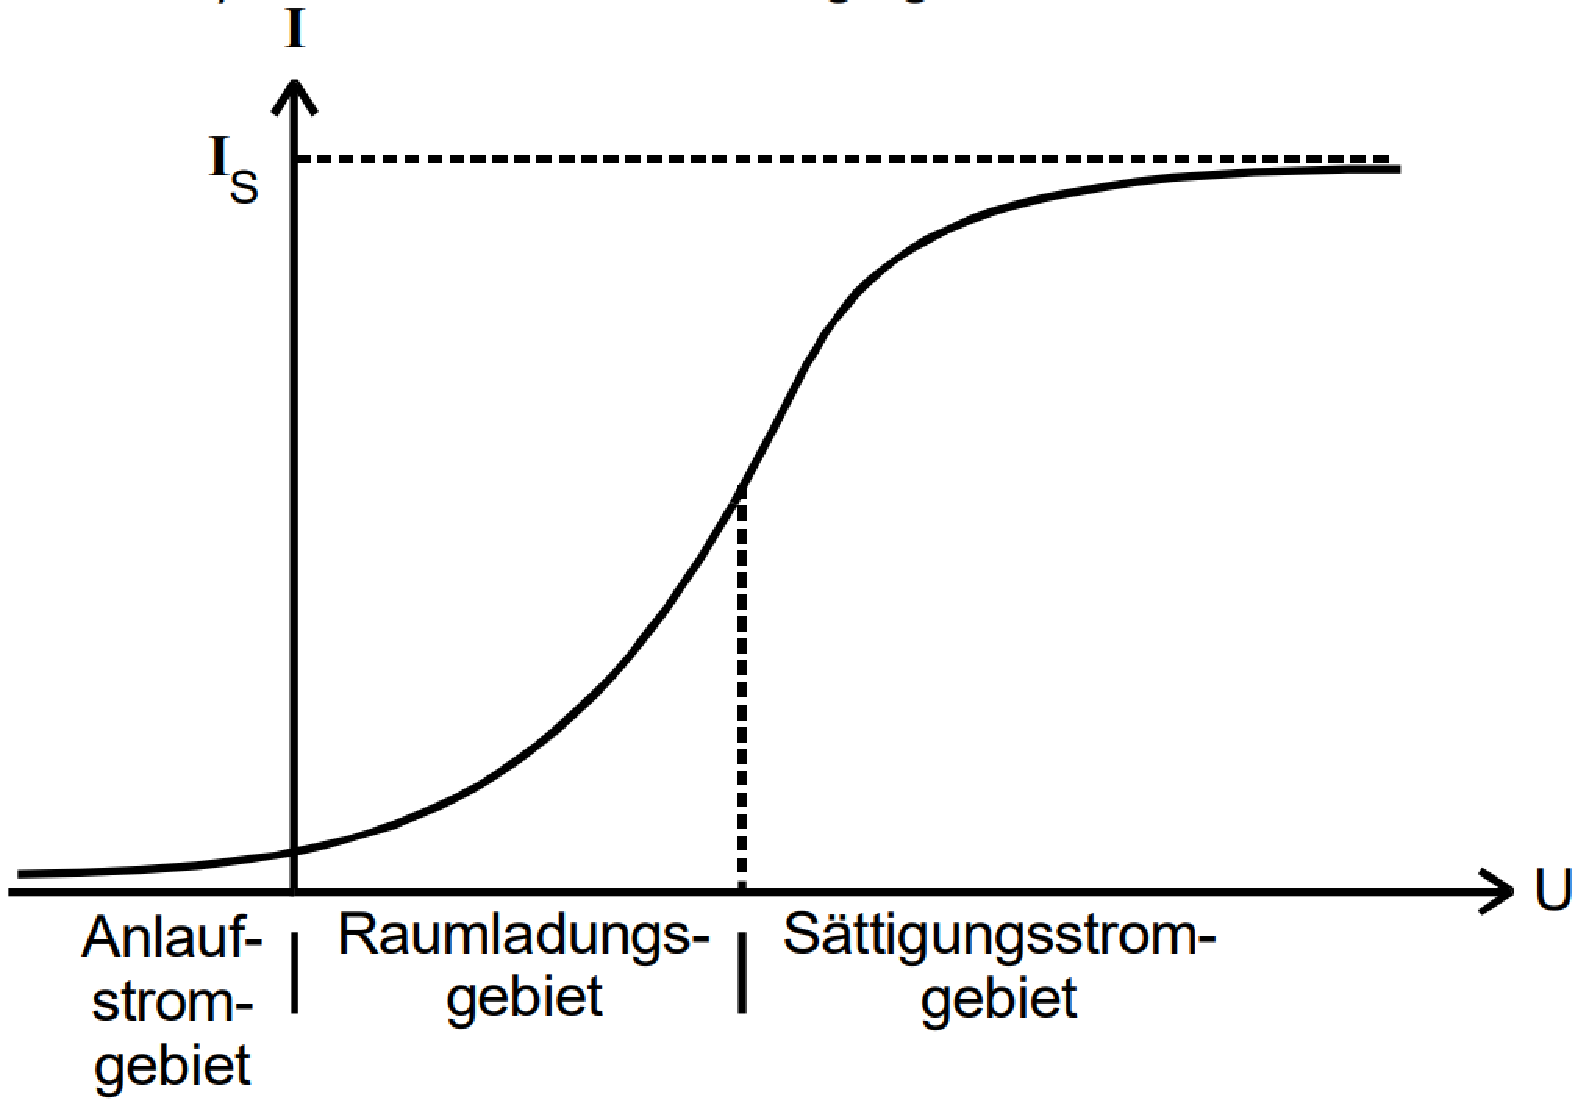
\includegraphics[width=0.5\linewidth]{pictures/KennlinieTheorie.pdf}
\end{figure}
Durch die sogenannte Kennlinie lässt sich ein Zusammenhanf zwischen der Stromdichte $j / I_A$ und dem angelegten Potential
grafisch darstellen.
Eine theoretische Kennlinie würde wie in \hyperref[fig:KennlinieTheorie]{Abbildung \ref{fig:KennlinieTheorie}} aussehen.
Wie bereits in der \hyperref[fig:KennlinieTheorie]{Abbildung \ref{fig:KennlinieTheorie}} zu erkennen, lässt sich diese Kurve in drei Bereiche einteilen.
Das ist einmal das Anlaufstromgebiet, das Raumladungsgebiet ($\sim V^{\frac{3}{2}}$) und das Sättigungsstromgebiet.